\documentclass[../../main.tex]{subfiles}

\begin{document}
\section{Cache and Main Memory}
\subsection{How do bandwidth-bound computations differ from
compute-bound computations?}
The difference is quite obvious. When running a program, it will run in a finite amount of time (hopefully). But why doesn't it terminate instantly? What a silly question, because a computer has to execute one instruction at a time, and each instruction takes a little bit of time to complete.

Now, we differentiate between two kinds of operations: Usual CPU instructions and memory operations. The reason for this is that memory operations are relatively much more time expensive, and the recent hardware trends make this gap grow bigger. Hence, we would like to know whether our program is bottlenecked by these expensive memory operations, which we very much would like to avoid, as we want to utilize our CPU with useful instructions instead.

To this end, we call computations \em memory-bound \em iff they are bottlenecked by the latency of memory operations. This, of course, is dependent on many factors, such as hardware and so on.

If our program is not memory-bound, it still executes not instantly, as it is bound by the execution speed of the CPU. We have a \em compute-bound\em . In a sense, every program or operation experiences a compute-bound. Hence, it is more useful when we quantify this bound, by analyzing the CPU frequency and the execution speed of individual operations, so that we can estimate the program's execution time.

\bigskip
\subsection{Influence of temporal locality and spatial locality on program performance}
If our program uses a lot of data, and thus faces a memory-bound, we have to intentionally engineer a program that employs good temporal as well spatial locality.

This is, because a lot of data will be read from and written to memory, which, as explained, is very time consuming. Luckily, computer engineers introduced caches to this end, which store some data of main memory, and provide it to the program with faster access times. The only problem will be if the caches, or, more precisely, their hash bucket are full. Because caches are usually not \em fully-associative\em , which means that if we have a cache line in memory, we can not write it to any cache line in the cache as we like. In fact, we only have $N$ cache lines available in an \em N-way associative \em cache.

As we can see, caches are very useful, but we have to understand their behavior in order to specifically tailor a program to effectively utilize them. In fact, a \em cache-aware \em algorithm employs good temporal as well as spatial locality. But what does that mean?

\begin{description}
    \item[Temporal locality] describes the concept that recently accessed memory has a higher probability to be accessed again.
    \item[Spatial locality] on the other hand is used to refer to the concept that memory, which is spatially close to recently accessed memory, has a higher probability of being accessed itself.
\end{description}

\noindent
But why is all that useful? Well, it is due to the \em replacement policy \em of caches. As explained, caches will run full, and at that instance, they will have to evict a cache line. But how do they decide? Well, one common replacement policy is \em LRU (Least Recently Used)\em , which means that they choose the cache line whose access is the most far away in time. This is why temporal locality comes in handy, as it increases the chances that our data lies in cache, and thus reduces the risk of a cache miss.

Finally, spatial locality is useful, because, as described, caches hold entire cache lines, which commonly hold 64 bytes of memory. Hence, if the data we access is closely clustered, we reduce the potential number of cache lines required, reducing the space requirement in the cache, and we will have more accesses to our cache lines. All of this contributes to a lower risk of a cache miss, which ultimately reduces the running time of our program.

\bigskip
\subsection{Cache Associativity}
On the slides 15 and 17 we hear about caches being \em N-way associative\em . Let's investigate on this topic further. Let's analyze the following picture (from Wikipedia):

\begin{figure}[ht]
    \centering
    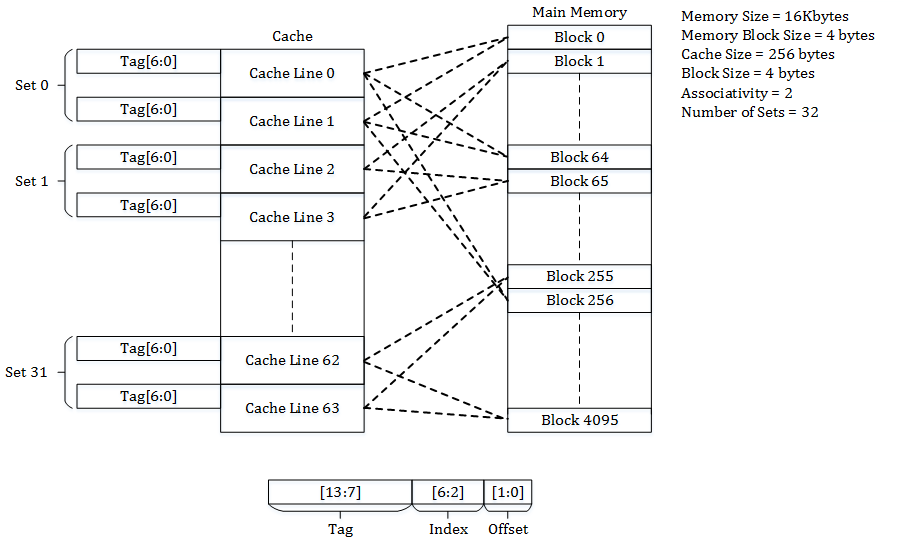
\includegraphics[width=\linewidth]{chapters/09/Set-Associative_Cache_Snehal_Img.png}
    \caption~{2-way associative cache \footnotemark}
    \label{fig:example}
\end{figure}
\footnotetext{Image source: \href{https://en.wikipedia.org/wiki/Cache\_placement\_policies\#/media/File:Set-Associative\_Cache\_Snehal\_Img.png}{https://en.wikipedia.org/wiki/Cache\_placement\_policies\#/media/File:Set-Associative\_Cache\_Snehal\_Img.png}}

~\\
Since this cache is 2-way associative, two consecutive cache lines form a group. For example, cache line 0 and 1 both belong to group 0. If we both know the $cache\_line\_size$ and the $cache\_size$, we can calculate $no\_cache\_lines = \frac{cache\_size}{cache\_line\_size}$. Now, we can calculate the number of sets these cache lines form because of associativity: $no\_sets = \frac{no\_cache\_lines}{N}$.

~\\
Now, here comes the clever part. When determining the memory address of the stored data in the cache, we can save 5 bits in this example, as this information is stored in the index of the block. More precisely, we have $no\_index\_bits = \log_2(no\_sets)$. The offset determines the exact location inside the cache line, and hence $no\_offset\_bits = \log_2(cache\_line\_size)$.

~\\
Finally, the remaining bits that are needed to uniquely identify the memory address are grouped into the \em Tag\em . How many bits do we need exactly? Well, here is one explanation: In total, there are $no\_address\_bits = \log_2(memory\_size)$ bits needed. But we already have \em index \em and \em offset \em bits, so there are $no\_tag\_bits = no\_address\_bits - (no\_index\_bits + no\_offset\_bits)$ bits remaining.

\bigskip
\subsection{An Overview of Cache Optimization Techniques and Cache-Aware Numerical Algorithms}
In this paper the author explains the importance of cache-aware programs, as compilers won't help us much in this regard. Hence, let's investigate on some practical examples where we can improve temporal and / or spatial locality.

\begin{description}
    \item[Loop Blocking] This is best understood by an example. Say we have the following code:
    
    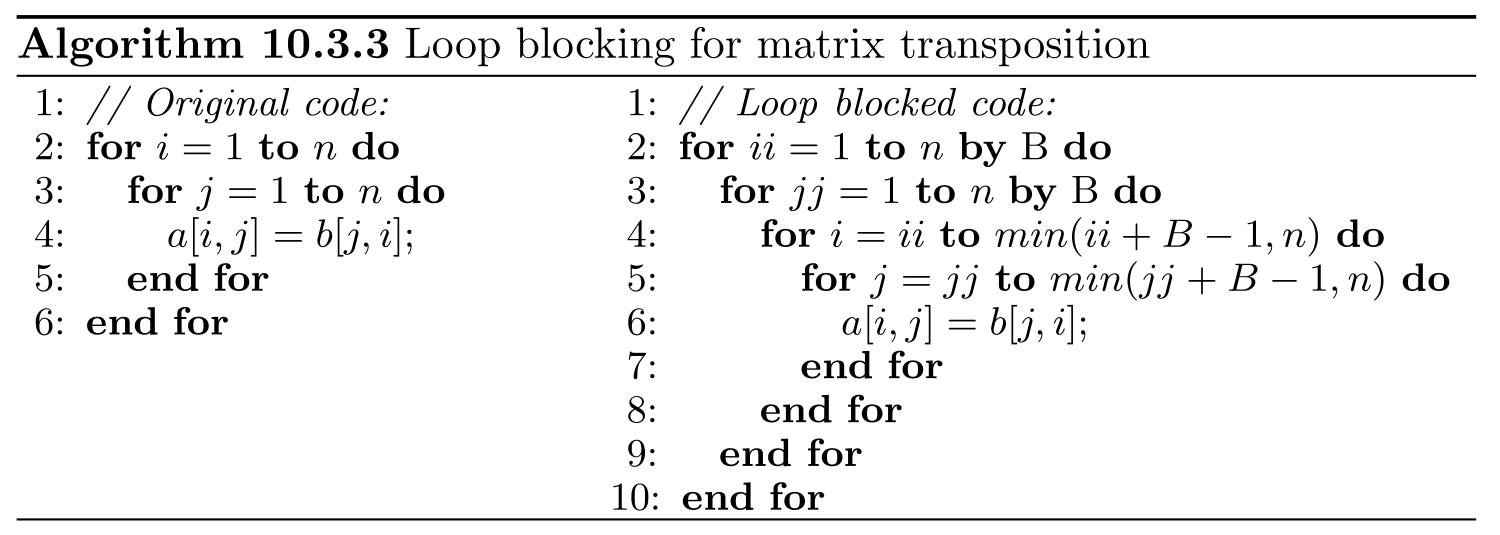
\includegraphics[width=\linewidth]{chapters/09/loop_blocking.png}

    Both matrices $a$ and $b$ are stored in row-order fashion. Hence, when running the left algorithm, $a$ has good spatial locality, whereas $b$'s is horrendous, as it leads to a cache miss on every access. The idea now is to find a tradeoff between these two. Let us analyze the access pattern of the two algorithms:

    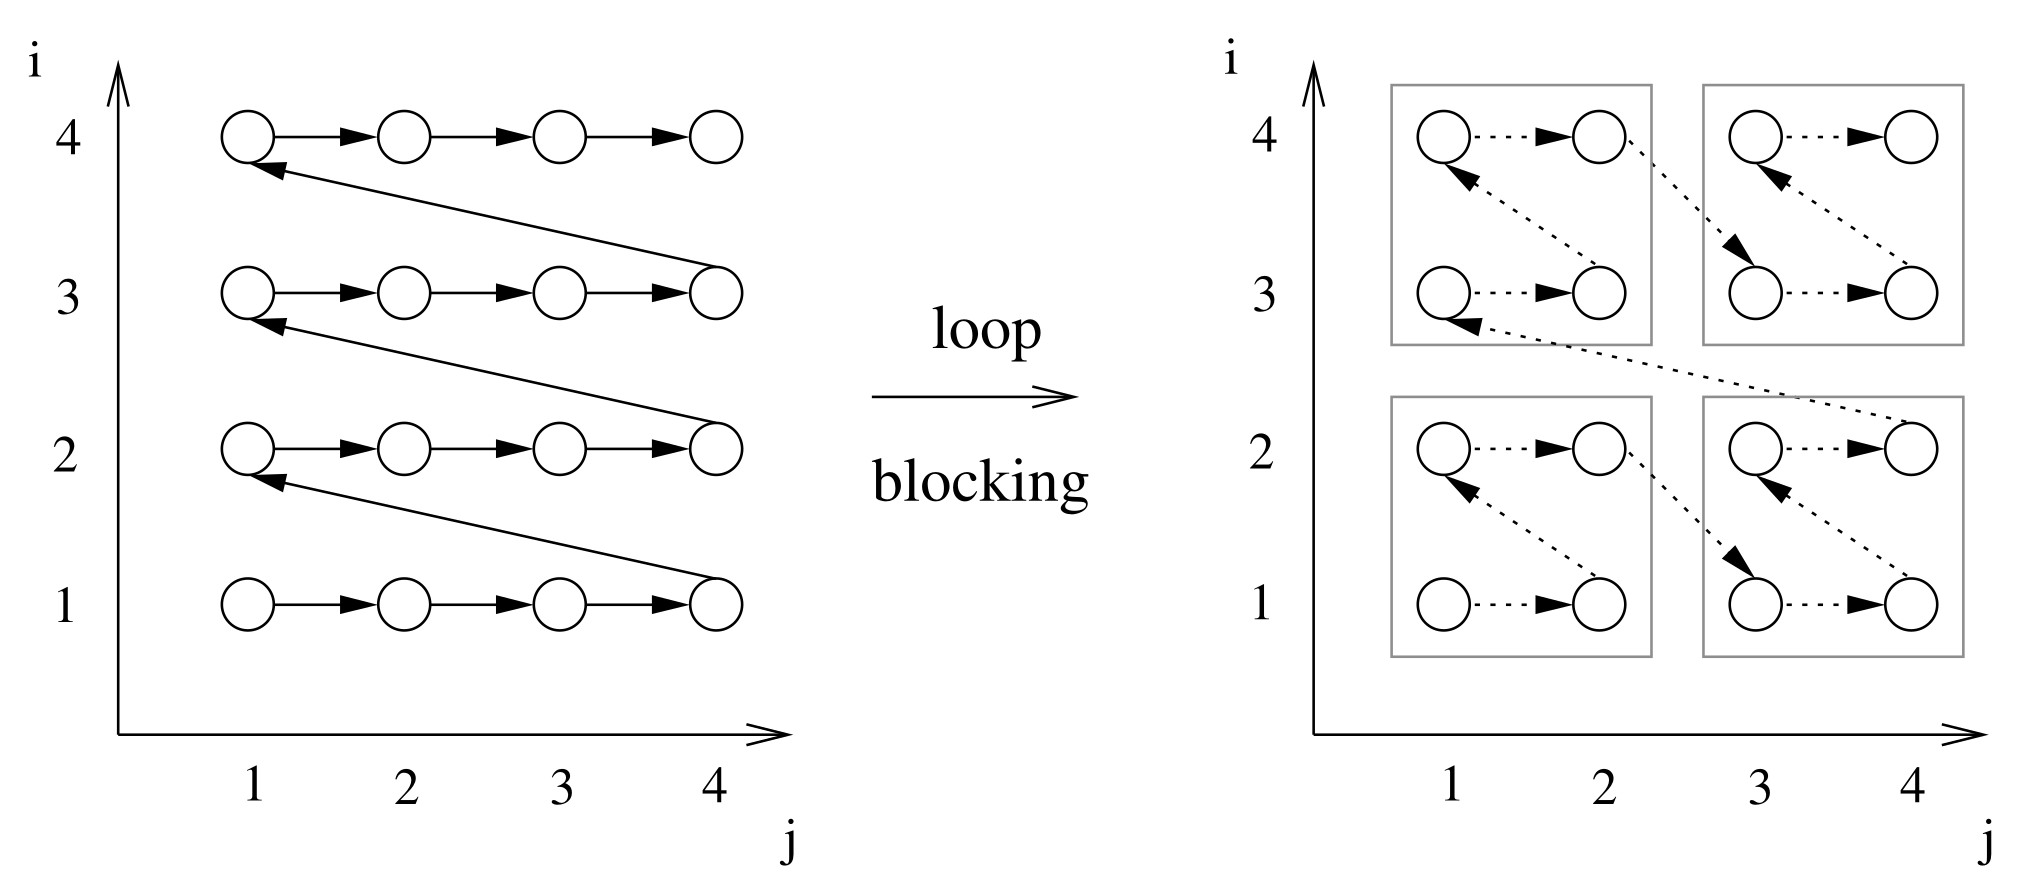
\includegraphics[width=\linewidth]{chapters/09/access_pattern.png}

    Note that walking along the rows is good for spatial locality, and also note that for b the graphic should be flipped along $y=x$.

    So why is the right access pattern better? Note the following: for $a$, the spatial locality does get a bit worse, but only in $O(1)$ fashion, as now we have to maybe load two more cache lines into the cache, not really a big deal. But what about $b$? Well, it basically divides its cache misses by a factor of 2 (in case of a block size of 2)! Thus, the overall cache misses will be reduced.

    \item[Array Padding] This one is rather specific, but it is quite useful to keep it in the back of one's mind. Imagine for the sake of argument that we have cache which can hold 1024 doubles in total, and has a 1-way associative cache (we will now see why this is maybe a bit too aggressive). Next, consider this algorithm:
    
    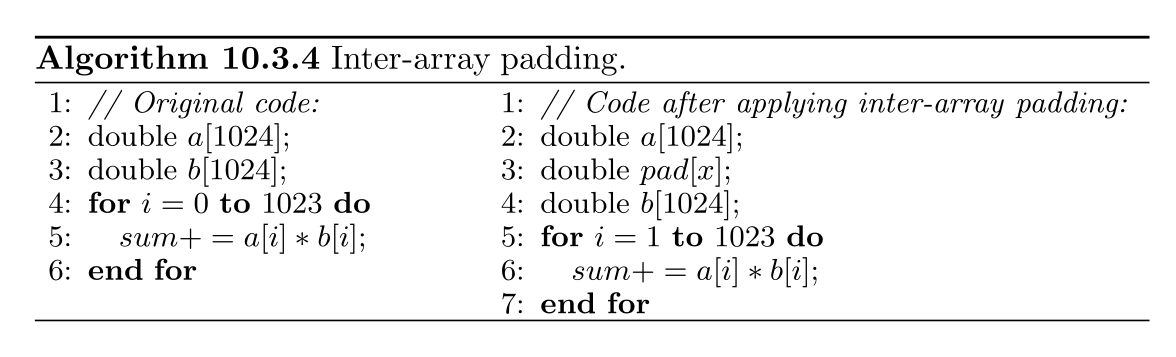
\includegraphics[width=\linewidth]{chapters/09/array_padding.png}
    
    It just so happens that in this instance both array $a$ and $b$ will map to the same cache lines (compare to my previous explanation). But, as there is only one slot in the cache for a specific cache line with a certain index, we will load a cache line of array $a$, right after that we will evict it for $b$, and then again for $a$ and so on. In the end, we will have a cache miss on every access, yikes. If only the cache line indices of $a$ and $b$ wouldn't align. Well, exactly this is the idea behind the algorithm on the right: We simply occupy some padding space in-between the two arrays, which the cache will be grateful for.

    This example was obviously very specific, but we can see that we might have to be a bit more careful if we had large arrays, maybe multiple of them, which in memory are separated by a large power of 2.
\end{description}
\end{document}